\documentclass[conference]{IEEEtran}
\usepackage[utf8]{inputenc}
\usepackage[T1]{fontenc}
\usepackage{booktabs}
\usepackage{amsmath,amssymb}
\usepackage{graphicx}
\usepackage{microtype}
\usepackage{url}
\usepackage[hidelinks]{hyperref}
\usepackage{cite}

\newcommand{\noteExternalVsRepaired}{%
$\blacktriangledown$ adjusted simultaneous interval entirely below zero (the arm recovers \emph{less} than \texttt{riv16-C1}); $\blacktriangle$ entirely above. Residence is a \emph{log loss} difference, so a positive value means the arm supplies \emph{less} residence capability. ACS 2018 development pools; three seeds. The last column counts seeds clearing the legacy service-probe allowance, out of 3 (\texttt{riv16-C1} clears 1/3).%
}

\newcommand{\noteRepairDiagnostic}{%
The upper rows are a diagnostic of the \emph{objective}; the lower block is a measurement of the \emph{release}. They are reported separately because an exactly invariant objective did not produce less measured disclosure. The attained rotation share is not a supremum -- every rotation search stopped on budget exhaustion or a failed line search -- and it is not a causal decomposition of what the optimiser did.%
}

\newcommand{\noteExternalVsJ}{%
A blank cell is an \textbf{unresolved} difference at three seeds, not a demonstrated equality: the adjusted interval contains zero and also contains effects of the size this table reports elsewhere. No equivalence or non-inferiority test was run for these cells. Negative residence means the arm supplies \emph{more} residence capability than $J$.%
}

\newcommand{\noteRelatedWork}{%
\checkmark\ the text demonstrates it; -- its setting excludes it; \textquotedblleft part.\textquotedblright\ a partial form (an adversarial objective or a transfer test, not an independent attacker slate); \textsc{unv.}\ could not be settled from what was read and is \textbf{not} guessed from a title or abstract. Several of these methods can be \emph{adapted} into this setting; three were, and they beat the mechanism developed here. Provenance for every row, including which sources were read in full text and which only as abstracts, is in \texttt{RELATED\_WORK\_COMPARISON.md}.%
}


\begin{document}

\title{Releasing a Feature Channel Beside a Prediction Service You Cannot Change:\\
An Evaluated Release Problem and Six Negative Mechanism Results}

\author{\IEEEauthorblockN{Anonymous Submission}}

\maketitle

\begin{abstract}
An organisation already publishes a prediction service: fixed probability vectors that downstream
recipients consume and cannot be asked to re-accept. We formalise and evaluate what happens when it adds
a second, reusable feature channel for one recipient without altering a published number, while limiting
what that recipient, and that recipient colluding with another, can newly infer about sex and race. Our
contribution is an implemented release interface and measurement contract: per-recipient and coalition
views, independently fitted attackers, incremental disclosure reported beside absolute disclosure, and
negative increments retained unclipped. On a locked, previously unused survey year, a penalty built from
the coalition's joint view beats an equal-strength and an equal-total-mass local control on 14 of 16
sensitive cells, none worse; its utility cost is bounded by a point rule, not by an interval. Six
subsequent mechanisms fail to improve on the strongest channel we already had, under both registered
senses of competitiveness: lower disclosure at comparable utility, and higher utility at bounded
disclosure. Adapted published erasers beat our own mechanism. A capacity diagnostic then shows why the
most recent attempt could not have succeeded as designed: a label-free code of the permitted inputs
carries genuine signal for the held-out task, yet adds nothing measurable once the already-released
service predictions are in the view---a result about appending, not about replacing. We report the release problem, the evaluation design, and every
claim this revision withdraws.
\end{abstract}

\section{Introduction}

A company runs two prediction services. One returns credit-style probabilities to a business partner;
the other returns coverage probabilities to a different partner. Both partners have built systems on
those exact numbers, so the company cannot revise them. It now wants to give the first partner something
more useful---a compact reusable feature vector built from what the published predictions leave
unexplained---while making sure that the partner, and the two partners pooling what they hold, cannot use
it to work out an applicant's sex or race any better than the published predictions already allow.

That situation is ordinary and it is not what the fairness and concept-erasure literature usually
evaluates. Most methods assume the releaser owns the representation and may edit or replace it. Here the
published output is immutable: it is already in the recipients' systems, and the only decision left is
what to put \emph{beside} it. That constraint changes what a mechanism may do, what preservation means,
and who the adversary is.

This paper contributes the problem, an implemented interface for it, a measurement contract, and the
results of six mechanisms evaluated through them. One effect replicates on a sealed year. Every mechanism
we built to turn that effect into a competitive release failed, and three adapted published erasers beat
our own mechanism on the same wire. We report that plainly, because the evaluation design is what makes
the failures legible, and because the negative results are specific enough to constrain what should be
tried next.

\paragraph*{Contributions}
\begin{itemize}\itemsep2pt
\item \textbf{A release problem with an immutable published output}, formalised with per-recipient and
coalition audit views, and an interface in which preservation is a bitwise identity rather than a bounded
perturbation (\S\ref{sec:interface}).
\item \textbf{A measurement contract} that makes heterogeneous mechanisms comparable at matched width on
one wire: independently fitted attacker slates, incremental disclosure always reported beside absolute
disclosure, negative increments retained unclipped, per-endpoint results never averaged
(\S\ref{sec:interface}).
\item \textbf{One confirmed effect} on a locked, previously unused survey year: coalition-conditioned
penalties beat both matched local controls (\S\ref{sec:confirmed}).
\item \textbf{Six negative mechanism results} against the strongest channel we had, under both registered
senses of competitiveness, with adapted published erasers outperforming our mechanism
(\S\ref{sec:negative}).
\item \textbf{A capacity diagnostic} explaining why the most recent design could not have worked as
specified, and a delimitation of exactly what it rejects (\S\ref{sec:capacity}).
\end{itemize}

\textbf{What this paper is not.} It does not present a deployable competitive mechanism; we do not have
one. It offers no new mathematics: concept erasure, eigenvalue-sign rank selection, minimax adversarial
training and conditional-moment characterisations are prior work, cited as such, and adversarially
protected transferable representations are not new either~\cite{madras2018laftr}. The framework does not
establish a superior method, and we do not claim that it does.

\section{The interface and the measurement contract}
\label{sec:interface}

Each person has covariates $X$, sensitive attributes $S$ (sex, 2 classes; race, 9 classes) and task
labels. Two services are frozen and published before anything else happens: $H_A(X)\in[0,1]^4$, the
income-over-\$50k and employment probability vectors released to recipient~A, and $H_B(X)\in[0,1]^2$, the
coverage vector released to B. A mechanism may add a channel $Z\in\mathbb{R}^{16}$ \emph{for A only}, so
A sees $(H_A,Z)$, B sees $H_B$, and the coalition AB sees $(H_A,Z,H_B)$. $H$ without a subscript is the
no-channel interface. The policy authorises A for income, employment and residence, and B for coverage
and commute; sex and race are forbidden everywhere, along with nine cross-role combinations. The
adversary holds labelled data from the release year, fits fixed attack families on its own pool, selects
on a validation pool, and sees only its legal view. Inference for A uses A-side inputs only; $H_B$ enters
fitting and auditing and is never an inference input.

Three names recur. $A_0$ is an unprotected neural channel. \textbf{$J$} is an adversarially trained
16-dimensional channel from earlier work in this line, never retrained; it is the strongest comparator
here, and it is \emph{internal}---an experimental artifact of this project, not a deployed product
(\S\ref{sec:contract}). $L1$ and $L2$ are local controls whose penalty uses only A's own view, matched to
the candidate on penalty strength and on total penalty mass respectively; $C1$ adds a penalty term built
from the coalition's joint view.

\begin{figure*}[t]
\centering
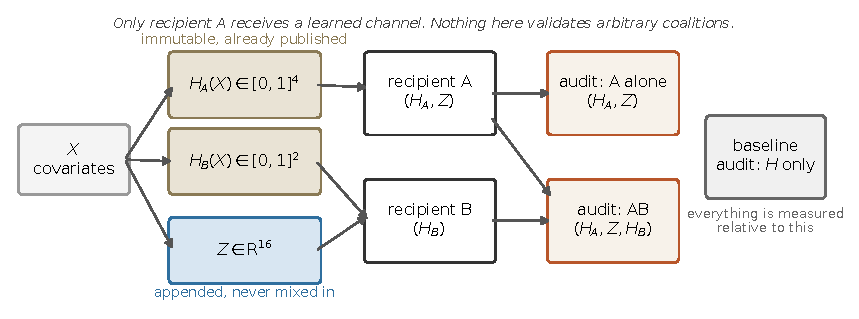
\includegraphics[width=0.86\textwidth]{figures/release_view.pdf}
\caption{The release graph. $H_A$ and $H_B$ are published and never modified; $Z$ is appended to A's wire
alone. Three audit views are scored: A alone, the coalition AB, and the $H$-only baseline that every
increment is measured against. A schematic, not a result.}
\label{fig:release}
\end{figure*}

Four distinctions carry the argument and are never merged.

\begin{itemize}\itemsep2pt
\item \textbf{Preservation is architectural; accuracy is empirical.} $Z$ is concatenated to $H_A$ and
never mixed into it, so $H$ is preserved by construction and checked bitwise on every released view. It
does \emph{not} follow that the service stays accurate: on identical released vectors, employment log
loss rises by $0.0138$ nats and income falls by $0.0145$ between two survey years.
\item \textbf{Added capability is measured against the correct $H$-only view.} A channel adds capability
only if independently fitted probes do better with $(H_A,Z)$ than with $H_A$ alone.
\item \textbf{Added disclosure is a finite-auditor log-loss gain, not an information bound.} Every
recovery number is the improvement a validation-selected attacker achieves over the same family
restricted to $H$. It is a floor on what is recoverable, never a ceiling.
\item \textbf{Recipients have different permitted tasks}, so the coalition's authorised union is not
either singleton's and the audit roles differ accordingly.
\end{itemize}

\textbf{Scope limits.} Only recipient A receives a channel, so nothing here is a multi-channel design.
Residence and commute labels are excluded from every representation fit and selection, but residence
outcomes have been inspected repeatedly across this line of work, so residence is \emph{reserved from
training} rather than a pristine unseen task, and we never describe a result on it as blind evaluation.

\textbf{Data and uncertainty.} California ACS one-year PUMS, ages 19--34, three household splits, with
disjoint pools for representation fitting, source validation, task fitting and validation, attacker
fitting and validation, and evaluation. Attacks are logistic regression, restarted MLPs, gradient-boosted
trees and a random-feature kernel family, plus every legal projection of $H$'s own attacks into each
view. Uncertainty is a paired household-cluster bootstrap with simultaneous intervals inside
pre-declared families. Both weightings (unweighted and person-weighted) are computed from the same
predictions and reported separately.

\section{What is proved, and over what}
\label{sec:proved}

Four statements are elementary; nothing else in this paper is a theorem.

\begin{enumerate}\itemsep2pt
\item Appending $Z$ without modifying $H$ preserves $H$ exactly. This is a property of concatenation.
\item \textbf{Inclusion fact.} A recipient holding $[H,Z]$ can ignore $Z$, so its optimal \emph{population}
log loss is no worse than with $H$ alone --- for the task \emph{and} for a sensitive attribute. A
deterministic appended channel therefore cannot reduce optimal sensitive recovery, and a constant
appended channel has exactly zero population incremental disclosure. Any reading of ``appending this
channel protected us'' is wrong by construction; only finite fitted probes can move either way, and some
of our measured increments are negative.
\item Under Bayes prediction and log loss, the population risk difference between $H$ and $(H,Z)$ equals
$I(S;Z\mid H)$. Our validation-selected finite attackers do not attain those infima, so reported
differences bound that quantity in neither direction, and mutual-information estimation has its own
formal limits~\cite{mcallester2020formal}.
\item For one refinement, orthogonal reparameterisation leaves the objective invariant, measured to
$5.6\times10^{-17}$.
\end{enumerate}

Ky Fan's principle~\cite{fan1949weyl} gives a restricted optimum for the original fixed-matrix family
only; the refinements have no fixed matrix and inherit no optimality statement. The moment condition we
use is a finite fitted subset of the $L^2$ characterisation of conditional independence behind kernel CI
tests~\cite{zhang2011kci,strobl2019rcit}. Vanishing fitted moments establish no conditional independence:
one of our own fixtures has a misspecified nuisance manufacturing a penalty more than ten times the
oracle value under \emph{exact} conditional independence.

\section{Related work}
\label{sec:related}

The closed-form line of Sadeghi et al.\ solves this shape of problem when the releaser owns the
representation: SARL~\cite{sadeghi2019sarl} takes eigenvectors of a utility-minus-$\lambda$-dependence
matrix, OptNet-ARL~\cite{sadeghi2021optnetarl} embeds closed-form players in a learned encoder,
K-TOpt~\cite{sadeghi2022ktopt} adds random features and evaluates on Folktables~\cite{ding2021retiring},
and U-FaTE~\cite{dehdashtian2024ufate} adds a conditional penalty. Our marginal arms turn out to
\emph{be} SARL-style constructions on whitened residuals, verified by bitwise rebuild. Adversarial fair
and transferable representation learning is Madras et al.~\cite{madras2018laftr}. Linear concept
erasure~\cite{belrose2023leace,holstege2025splince} gives an exact guarantee against \emph{linear}
adversaries on a representation the releaser may edit. Adversarial removal is known to leave recoverable
information~\cite{elazar2018adversarial}, and least-privilege learning has fundamental
limits~\cite{stadler2024leastprivilege}. \textbf{Reusing a known solver, a conditional-moment
characterisation or a rank rule is attribution, not innovation.}

Three things differ here, with their weight stated honestly. \emph{What we condition on}: a released
continuous artifact $H$, through cross-fitted nuisance residuals, rather than stratification on a label.
\emph{What utility means}: reconstruction of a residualised teacher rather than dependence with a label.
\emph{Recipient structure}: separate local and coalition penalties over a fixed prior output, with only
one recipient receiving a channel. The first two are adaptations of known components. For the third, the
nearest prior candidate we found is the multi-consumer information-theoretic
line~\cite{sankar2013utility}, which designs one sanitised release consumed by many users; we could not
confirm from its text that it carries a per-recipient release or a collusion term, and we mark that entry
ambiguous rather than assert it. What we did not find, after a bounded search, is a prior
\emph{evaluation} of recipient-specific and combined-access policies over an already-published output the
mechanism may not touch. That is absence of evidence, not a priority claim.

\section{The confirmed effect}
\label{sec:confirmed}

\begin{figure*}[t]
\centering

\includegraphics[width=\textwidth]{figures/forest_primary.pdf}
\caption{Paired differences with simultaneous $95\%$ intervals inside each pre-declared family, fresh
attacks on the locked year, both weightings, candidate minus comparator in nats. \textbf{Left:} the
coalition-conditioned candidate against its two local controls. The two grey A/sex rows are
\emph{unresolved}---the comparison is undecided, not the endpoint unaffected. \textbf{Right:} the same
candidate against the frozen channel $J$.}
\label{fig:forest}
\end{figure*}

On a locked survey year that no earlier stage of this project had touched, the coalition-conditioned
candidate $C1$ has a simultaneous-interval advantage over both $L1$ and $L2$ under both weightings. Of
the 16 sensitive cells, \textbf{14 have adjusted intervals entirely below zero, none is above zero, and
two are unresolved} ($C1$ versus $L1$ on A/sex unweighted, $[-0.00585,+0.00020]$; versus $L2$,
$[-0.00568,+0.00052]$). Frozen attacks from the earlier year reproduce the ordering, so this is not an
artifact of refitting attackers on the new year.

Two qualifications travel with that result and are not separable from it. First, \textbf{the paired
utility rule is a point criterion and only a point criterion}: as implemented it compares seed means at a
$0.001$-nat margin and passes, but \textbf{zero of four comparisons support interval non-inferiority at
that margin}, missing it by $2\%$ to $35\%$ even under the most permissive procedure we computed. ``No
statistically detected cost'' and ``a cost bounded below $0.001$'' are different statements and only the
first is supported. Second, \textbf{the mechanism is not competitive with $J$}: $C1$ is significantly
worse than $J$ on all four sensitive endpoints under both weightings, and better only on residence
capability. Since $J$ carries materially less residence capability than the spectral arms, neither
channel dominates the other.

\section{Six mechanisms that did not improve on \texorpdfstring{$J$}{J}}
\label{sec:negative}

We group the negative results by what they tested rather than by the order they ran; the chronology, with
evidence commits, is in Appendix~\ref{app:chronology}.

\subsection{Refining the penalty}
A penalty acting on nonlinear functions of the channel moved recovery in the intended direction but
failed all eight registered coordination cells, and at reduced rank it made one endpoint significantly
\emph{worse} ($+0.00862\,[+0.00168,+0.01556]$). That penalty was then diagnosed, after its maps had been
evaluated, as coordinate-dependent: it summed degree-two monomials with equal weight instead of computing
a Frobenius norm. A successor objective repaired that exactly---rotation-only share $1.4\times10^{-15}$
over 18 cells, verified before any score was read---and \textbf{the repaired releases disclosed more}: 8
of 48 sensitive cells significantly worse, none better. The repair changed five ingredients at once, so
no single cause is isolated, and we do not claim that rotation invariance is harmful.

\subsection{Published erasers, adapted, beat our mechanism}
\label{sec:external}
LEACE~\cite{belrose2023leace} and SPLINCE~\cite{holstege2025splince} were applied to the auxiliary
channel alone and appended to unchanged $H_A$; they are deliberately \emph{not} applied to the
concatenated wire, since an oblique projection over all coordinates would generally change the published
service output. Adapted LEACE and two OptNet-ARL policies recover significantly less than our repaired
mechanism on all four sensitive endpoints under both weightings, and adapted SPLINCE on seven of eight
cells (Table~\ref{tab:extrep}). \textbf{A closed-form linear eraser from 2023, applied to a channel this
project already had, beats the mechanism this line of work developed across three studies.} The utility
side must be stated with equal care: LEACE's residence cost against the repaired arm is
\emph{unresolved}, $+0.0036\,[-0.0028,+0.0100]$, and against the channel it actually transformed it is
significant, $+0.0098\,[+0.0036,+0.0159]$. Linear erasure of this channel buys its protection with
measurable authorised capability, so we do not say it dominates.

\begin{table*}[t]
\centering\footnotesize
\begin{tabular}{@{}llcccccc@{}}
\toprule
& & \multicolumn{4}{c}{additional recovery vs.\ \texttt{riv16-C1}} & residence & source \\
\cmidrule(lr){3-6}
Arm & wt. & A / sex & AB / sex & A / race & AB / race & loss diff. & allow. \\
\midrule
\texttt{LEACE} & unw. & $-$0.0081$\blacktriangledown$ & $-$0.0086$\blacktriangledown$ & $-$0.0131$\blacktriangledown$ & $-$0.0158$\blacktriangledown$ & +0.0036 & 3/3 \\
 & PWGTP & $-$0.0097$\blacktriangledown$ & $-$0.0093$\blacktriangledown$ & $-$0.0154$\blacktriangledown$ & $-$0.0166$\blacktriangledown$ & +0.0040 &  \\
\addlinespace[1pt]
\texttt{SPLINCE} & unw. & $-$0.0088$\blacktriangledown$ & $-$0.0077$\blacktriangledown$ & $-$0.0183$\blacktriangledown$ & $-$0.0165$\blacktriangledown$ & +0.0089$\blacktriangle$ & 3/3 \\
 & PWGTP & $-$0.0100$\blacktriangledown$ & $-$0.0084 & $-$0.0201$\blacktriangledown$ & $-$0.0163$\blacktriangledown$ & +0.0091$\blacktriangle$ &  \\
\addlinespace[1pt]
\texttt{OptNet-C1} & unw. & $-$0.0074$\blacktriangledown$ & $-$0.0110$\blacktriangledown$ & $-$0.0161$\blacktriangledown$ & $-$0.0145$\blacktriangledown$ & +0.0086$\blacktriangle$ & 2/3 \\
 & PWGTP & $-$0.0089$\blacktriangledown$ & $-$0.0117$\blacktriangledown$ & $-$0.0183$\blacktriangledown$ & $-$0.0151$\blacktriangledown$ & +0.0076$\blacktriangle$ &  \\
\addlinespace[1pt]
\texttt{OptNet-L1} & unw. & $-$0.0032 & $-$0.0048 & $-$0.0056 & $-$0.0060 & +0.0057 & 2/3 \\
 & PWGTP & $-$0.0059 & $-$0.0069 & $-$0.0116 & $-$0.0075 & +0.0046 &  \\
\addlinespace[1pt]
\texttt{OptNet-L2} & unw. & $-$0.0104$\blacktriangledown$ & $-$0.0092$\blacktriangledown$ & $-$0.0184$\blacktriangledown$ & $-$0.0198$\blacktriangledown$ & +0.0096$\blacktriangle$ & 2/3 \\
 & PWGTP & $-$0.0125$\blacktriangledown$ & $-$0.0112$\blacktriangledown$ & $-$0.0210$\blacktriangledown$ & $-$0.0212$\blacktriangledown$ & +0.0082$\blacktriangle$ &  \\
\addlinespace[1pt]
\bottomrule
\end{tabular}

\caption{Adapted published methods against the repaired mechanism at rank 16 with the coalition policy.
Every arm transforms only the auxiliary channel and appends it to unchanged $H_A$. Development pools.
\noteExternalVsRepaired}
\label{tab:extrep}
\end{table*}

\subsection{Training the channel directly against attackers}
Direct adversarial refinement of the channel, starting from the unprotected channel $A_0$, produced 60
distinct new channels and improved no sensitive endpoint against any comparator: across its frontier
family 189 cells are significantly worse and 18 significantly better, \emph{all 18 on residence utility}.
Its one positive---that coalition conditioning beats a local control---survives robustly only against the
\emph{weak} control; against the strength-matched control it holds on one endpoint at one width at the
family-adjusted level and not under the simultaneous correction its negative results are held to. A
separate finding from the same study is worth more than its headline: 63 of 114 trajectories published a
checkpoint bitwise identical to their starting channel although every one had moved, so unchanged
releases were a \emph{selection} outcome, not stasis.

\subsection{Starting from \texorpdfstring{$J$}{J}, and projecting out of \texorpdfstring{$J$}{J}}
The most direct test initialised adversarial training from $J$'s own trained weights and, separately,
removed coalition-conditioned directions from $J$ by a rank-reducing projection. \textbf{No prospectively
selected release met the registered competitive conjunction} under either weighting. The neural nominees
\emph{are} $J$: at low teacher strength the registered equal-budget selection returned the untouched
starting channel on every anchor, and at higher teacher strength the channel was pulled back toward $A_0$
and leaked more. The projection nominees lower coalition sex recovery against $J$
($-0.0091\,[-0.0158,-0.0025]$) at a significant residence cost ($+0.0101\,[+0.0023,+0.0179]$ unweighted),
which is a trade-off rather than dominance, and they do not separate from matched local-only projections
on any endpoint---so coalition conditioning established no advantage here. Their point estimates sit
within $\pm0.0011$ of ordinary LEACE applied to $J$ on every endpoint unweighted, which is point
proximity and not statistical equivalence.

\subsection{Buying capability instead of lowering disclosure}
\label{sec:utilityfirst}
A release beside $H$ can be competitive in two ways: lower disclosure at comparable utility, or higher
utility at bounded disclosure. The studies above registered the first. A sixth registered the second:
append a small learned channel $R$ beside a frozen $J$, predicting residual teacher information a frozen
decoder from $(H_A,Z_J)$ leaves unexplained, and ask for capability at bounded added disclosure. Its
pilot passed the capability leg and the source allowances at every configuration and \textbf{failed the
declared $0.001$-nat disclosure screen at every configuration}; capability and disclosure fell together,
monotonically, as the adversarial weight rose (Fig.~\ref{fig:s6pilot}). The closest configuration missed
the screen at the lowest capability in the grid. Its expansion tiers were never triggered, and we report
them as such rather than as missing evidence.

\begin{figure*}[t]
\centering

\includegraphics[width=0.86\textwidth]{figures/study6_pilot.pdf}
\caption{Utility-first pilot (development pools): capability against the worst mean sensitive increment
over $J$, with the declared screen dashed. Increasing the adversarial weight moves each policy down and
to the left. Point-estimate screening values, not confidence statements.}
\label{fig:s6pilot}
\end{figure*}

\textbf{Label-free is not neutral.} The capability proxy uses no residential label, but it is the
residual of $A_0$, the unprotected channel that carries the largest sensitive recovery in this paper
($+0.032$ on A/sex and $+0.051$ on A/race over $H$). Rewarding reconstruction of that residual can reward
sensitive-correlated directions, so ``the objective itself paid for sensitive information'' remains a
live explanation of the pilot's inseparability, alongside ``no extension of $J$ in this family separates
them''. This design cannot distinguish them.

\section{A capacity diagnostic, and what it rejects}
\label{sec:capacity}

The most recent study asked whether a \emph{randomized} finite release, optimised under explicit
conditional-disclosure constraints, could reach an operating point the deterministic extension could not.
It registered a tier ladder with machine-readable gates and stopped at the first empirical gate.

\textbf{The stochastic solver was never run on data.} The finite-channel machinery was built and
validated on synthetic fixtures---where randomization does strictly beat the best deterministic
perfectly-private map---but no channel was ever constrained, fitted or audited on survey data, and no
cloud compute was spent. \textbf{This is therefore not a failed stochastic mechanism}, and nothing here
bears on whether a role-constrained stochastic release would beat a deterministic one. What failed is a
prior capacity question.

\textbf{What was measured.} A prespecified, label-free $k$-means code $T$ of the permitted A-side
inference inputs, at 64 states and at one predeclared 256-state fallback, was given to the house utility
probe family alongside the same-host $J$ release, and asked whether it retained a residence advantage
\emph{before} any privacy constraint. It did not: the anchor-mean advantage is $-0.00268$ nats at 64
codes and $-0.01136$ at 256, with no anchor positive under the unweighted accounting
(Table~\ref{tab:capacity}, Fig.~\ref{fig:capacity}). The gate failed and stages C and D did not run.

\begin{table}[t]
\centering\footnotesize
\begin{tabular}{@{}l r r r r@{}}
\toprule
code size & anchor & unweighted & person-weighted & paired SE \\
\midrule
$|T|=64$ & 0 & $-0.00091$ & $+0.00216$ & 0.00553 \\
 & 1 & $-0.00472$ & $-0.00400$ & 0.00479 \\
 & 2 & $-0.00241$ & $-0.00682$ & 0.00587 \\
\addlinespace[1pt]
\multicolumn{2}{@{}l}{\quad anchor mean} & $-0.00268$ & $-0.00288$ & \\
\midrule
$|T|=256$ & 0 & $-0.00404$ & $+0.00007$ & 0.00564 \\
 & 1 & $-0.01710$ & $-0.01315$ & 0.00557 \\
 & 2 & $-0.01295$ & $-0.01509$ & 0.00491 \\
\addlinespace[1pt]
\multicolumn{2}{@{}l}{\quad anchor mean} & $-0.01136$ & $-0.00939$ & \\
\bottomrule
\end{tabular}

\caption{Capacity diagnostic, development pools, validation split: residence advantage of
$[H_A,Z_J,\mathrm{onehot}(T)]$ over same-host $J$, per anchor and weighting, with the paired
household-bootstrap standard error. At $|T|=64$ every estimate lies within about one SE of zero: no
demonstrated advantage, and no demonstrated deficit.}
\label{tab:capacity}
\end{table}

\begin{figure}[t]
\centering
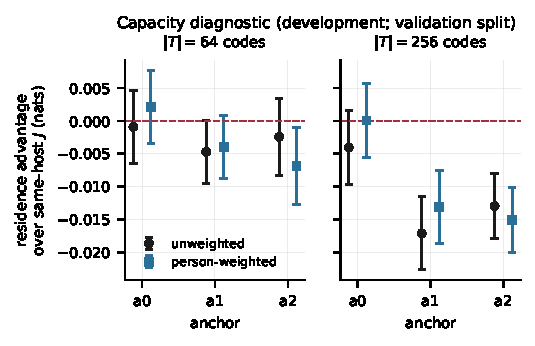
\includegraphics[width=\columnwidth]{figures/study7_capacity.pdf}
\caption{The same diagnostic with paired household-bootstrap standard errors. Development evidence on
repeatedly used pools; the test split was never read.}
\label{fig:capacity}
\end{figure}

\textbf{What the numbers support, and a reading we decline.} The code is not noise: alone it beats the
label prior in every anchor. Alone it is also beaten by $J$ in every anchor, and adding it to $J$ changes
nothing measurable (Table~\ref{tab:subsumption}). It is tempting to read that as the published service
predictions \emph{already carrying} whatever A-side residence signal exists, which would be a statement
about the release contract and a mechanism-level explanation for this line of work's repeated negatives.
\textbf{We decline that reading}, for two reasons. First, it does not follow from the measurement: the
differences are fractions of their own standard errors, and the comparison is one code at one
quantization resolution through one probe family (\S\ref{sec:capacity-limits}). Second, it conflates the
\emph{quantized code} with the A-side inputs it is built from---an unquantized view of those inputs is a
different object, and this diagnostic did not test one. A successor experiment separating quantization
loss from probe failure is registered and running; its outcome is not part of this paper, and we state
the distinction here rather than claim the explanation.

\begin{table}[t]
\centering\footnotesize
\begin{tabular}{@{}l r r r r@{}}
\toprule
anchor & prior$^\dagger$ & $T$ only$^\dagger$ & $J$ only & $J+T$ \\
\midrule
0 & 0.54501 & 0.53093 & \textbf{0.52507} & 0.52598 \\
1 & 0.52859 & 0.51292 & \textbf{0.50114} & 0.50586 \\
2 & 0.55554 & 0.53321 & \textbf{0.52856} & 0.53097 \\
\bottomrule
\end{tabular}

\caption{Residence validation log loss (nats, lower is better) at $|T|=64$. $^\dagger$The prior and
$T$-only columns are reported by the source study but have no machine-readable backing or committed
generator at the pinned commit; we report them as reported-not-verified. The $J$ and $J{+}T$ columns
reproduce exactly from its stored results.}
\label{tab:subsumption}
\end{table}

\subsection{What this diagnostic does not establish}
\label{sec:capacity-limits}

Four delimitations, each of which we enforce in the wording above.

\textbf{It is a fitted-probe result, not an information statement.} The differences that motivate it are
$0.16$, $0.98$ and $0.41$ standard errors from zero at the declared resolution, on 2048 fitting rows with
84 input columns against the baseline's 20, using a logistic and a 40-epoch MLP selected on validation
log loss. ``No measurable improvement at this probe capacity'' is supported; ``$T$ contains no useful
information beyond $J$'' is not. A probe family can miss information its own inputs jointly determine: in
an exact fixture with $Y=J\cdot T$ for independent signs, a score additive in $J$ and one-hot $T$ gains
exactly zero over the prior while the joint view determines $Y$. That is a capacity counterexample, not a
claim that residence behaves like this.

\textbf{It rejects appending, not replacing.} The diagnostic asks whether $T$ adds to $J$. It cannot see
a release that \emph{replaces} $J$. In an exact fixture with $H$ constant, $J=(Y,S)$ and $T=Y$ for
independent bits, appending $T$ to $J$ adds exactly zero task information, while replacing $J$ by $T$
preserves task utility in full and removes the sensitive bit entirely ($0.693$ nats of disclosure
removed). Append-redundancy is therefore not a universal rejection of replacement channels, and the
untested question---a prospective release beside unchanged $H$ for a new recipient, with $J$ as a
comparator rather than a component---remains open.

\textbf{It is one code, one probe family, two resolutions, three anchors}, on repeatedly used development
pools. It is not a capacity theorem and not a statement about the population. Higher resolution is
monotonically worse, which is consistent both with there being nothing to find and with the probe being
handicapped by width.

\textbf{One reported ceiling is withdrawn.} The study also estimated a fitted-model ceiling under a
partition it described as ``baseline probability deciles''. Those deciles are constructed from the
baseline probe's \emph{per-row log loss}, which is computed from each person's own residence label, so
the partition conditions on the outcome. The signature is visible in the numbers: ten cells take residence
log loss from about $0.52$ to $0.065$--$0.094$ nats. A fixture reproduces the effect on a label that is
pure noise at the same base rate: loss-decile conditioning ``predicts'' it at $0.057$ nats against a true
entropy of $0.590$, while the label-free control (deciles of the predicted probability) leaks nothing.
\textbf{We withdraw that estimate rather than reinterpret it}, and we use no ceiling in any claim here.
Its companion partition is label-free but has $1.9$--$2.1$ rows per cell and is unusable for a different
reason. Neither entered the gate decision, which rests on the deployable probe comparison alone; we
therefore do not propagate the defect to the gate outcome or to any other result.

\section{The release contract, and one assumption we could not verify}
\label{sec:contract}

The interface of \S\ref{sec:interface} says $H_A$ and $H_B$ are immutable published outputs. $J$ is
different: it is an experimental channel produced inside this project. In the source studies, ``released
wire'' denotes the experimental release interface---arrays written to disk and audited---not delivery to
an external recipient, and we found no evidence that $J$ was ever deployed to anyone.

This matters because the most recent design treated $J$ as a compulsory component of the new release, on
the stated ground that it ``was actually released to these recipients and remains accessible'' and so
could not be revoked. We could not substantiate that, and a later registration asserting prior deployment
is not evidence of deployment. The consequence is structural rather than cosmetic: holding $J$ inside the
release turned the capacity question into the append question of \S\ref{sec:capacity}, which is precisely
the question that cannot see a replacement win. \textbf{If the channel was never deployed, then $J$ is a
comparator and not a compulsory component}, and a release for a \emph{new} recipient under a prospective
contract is the natural next design. If deployment evidence exists, the old-recipient threat model
returns and must be audited as such; we state the dependency rather than resolve it by assumption.

\section{What this evidence does not establish}
\label{sec:limits}

\textbf{No attack maximum is an upper bound.} Every recovery number is what a validation-selected member
of a finite collection achieved. Three separate searches for a stronger attacker---a wider, deeper
network held out of every training ensemble, and two calibration suites---each failed to beat the
standard slate, which bounds what those searches found, not what exists.

\textbf{Development against confirmation.} Only the locked-year transport is confirmatory. The 2018 pools
have been used repeatedly, and three anchors with simultaneous intervals do not restore pristine
confirmation. A later survey year remains sealed and unscored: it has never been loaded, transformed,
inspected, scored or included in any restore bundle.

\textbf{Screening thresholds are not confidence statements.} Where a study nominated nothing, no adjusted
interval exists, and its pass/fail legs are point estimates.

\textbf{Precision near equality is limited.} On these endpoints and pools, an adjusted one-sided upper
bound at or below $0.001$ nats was not achievable for a comparison whose point estimate sat near zero:
the smallest adjusted half-width in the record is $0.00220$ nats and the medians run $0.0069$--$0.0136$.
This already holds unadjusted, so multiplicity is not the cause. It is a statement about \emph{those
comparisons in the near-equality regime}, not about the achievable precision of a mechanism that does not
yet exist: the standard error belongs to the paired per-household sensitive losses of a specific
comparison, and a release whose sensitive predictions nearly match the reference can have a much smaller
one while its task utility differs substantially.

\textbf{Audits do not transport across hardware below about $0.003$ nats}, because re-auditing refits the
attacker slate; comparisons are therefore made against same-host references and not differenced against
earlier published audits at finer precision.

\textbf{Machinery is itself an artifact.} One study's audit slate omitted the in-slate untouched-$J$
predictor its method text promised, so a safeguard was served by a differenced comparator instead; the
fix can only raise measured increments and therefore makes screens harder. Another study's training-time
penalty registers a positive gain for a provably non-disclosing constant channel, which affects the
interpretation of its weight knob rather than its audited leakage; its magnitude in that study is
unmeasured rather than estimated.

\textbf{Nothing here is a certificate.} Vanishing fitted moments imply neither conditional independence
nor any bound on $I(S;Z\mid H)$, and a guarantee in a fitted finite model is not a population guarantee:
in a validated fixture, binning a conditioning view drops a full $\log 2$ of measured leakage to exactly
zero.

\section{Open science}
\label{sec:openscience}

Every number in this paper is generated from committed evidence at pinned commits, and each printed digit
traces to a (commit, path, SHA-256) triple recorded in the submitted artifact. Table and figure
generators, the independent verification scripts, the claim ledger, the correction log and the
mathematical fixtures are included; no number was typed by hand. The evidence is ACS public-use
microdata, so no restricted data is redistributed. Anonymised artifacts will be shared within the
required window, and the final artifact deposited on acceptance.

\section{LLM usage considerations}
\label{sec:llm}

This work was substantially assisted by a large language model, and describing that as editorial help
would be inaccurate. A model was used to write and refactor experiment and analysis code, to draft and
revise this manuscript, to audit the studies' own reports against their source code and stored outputs,
and to construct the counterexample fixtures cited here. Experimental designs, registrations and stopping
rules were fixed in advance of outcomes and are committed; model-generated analyses were checked by
independently written scripts that recompute each reported quantity from the smallest machine-readable
source, and several claims in this paper exist \emph{because} that recomputation contradicted the
original write-up---the withdrawn ceiling of \S\ref{sec:capacity-limits} is one. The authors take full
responsibility for every claim, number and omission in the submitted work, including those first drafted
by a model; nothing was accepted on the model's assertion alone, and every load-bearing figure is
reproducible from the artifact.

\section{Conclusion}

A service that has already published predictions can add a reusable channel beside them without changing
a released number, and can steer that channel away from directions a recipient or a colluding pair would
use to infer sex and race. On a locked, previously unused year, coalition conditioning does what it
claims against both matched local controls, at a utility cost the data cannot bound below the margin its
rule used. Everything we built afterwards to make that into a competitive release failed, in both
registered senses of competitiveness, and adapted published erasers applied to a channel we already had
beat our own mechanism.

The most recent diagnostic narrows where to look next. A label-free code of the permitted inputs carries
real signal for the held-out task and adds nothing measurable once the published service predictions are
in the recipient's view---but at one quantization resolution, through one probe family, and with the
differences inside their own standard errors, which is not enough to conclude that the published output
already carries everything an extension could add. Two candidate explanations remain open and are
separable by experiment: quantization loss, and genuine redundancy with the published output. What the
evidence does say is that the append question and the replacement question are different, and that this
programme has so far measured only the first.

\textbf{The defensible contribution is the release problem and the evaluation design}: fixed published
outputs as a hard constraint, recipient-specific and coalition-specific audit roles, fresh and frozen
attackers never pooled, absolute and incremental recovery side by side, negative increments unclipped,
denominators beside every count, per-endpoint results never averaged, and a sealed temporal transport
with its multiplicity fixed in advance. That contract is what made six negative results legible instead
of ambiguous, and it is what we would keep.

\bibliographystyle{IEEEtran}
\bibliography{references}

\appendices

\section{Study chronology}
\label{app:chronology}
\begin{table*}[h]
\centering\footnotesize
\begin{tabular}{@{}l p{3.4cm} l l p{5.7cm}@{}}
\toprule
study & construction & evidence & status & what it established \\
\midrule
1 & locked ACS 2017 transport & \texttt{349efa45} & confirmatory & coalition effect over both local controls; the $.001$ point rule, not interval noninferiority \\
2 & nonlinear penalty / rank & \texttt{c37807e4} & development & negative; penalty coordinate-dependent, diagnosed after evaluation \\
3 & invariant repair $+$ external baselines & \texttt{73903b7f} & development & negative; closed-form erasers beat the developed mechanism \\
4 & direct adversarial refinement from $A_0$ & \texttt{69e790af} & development & negative on both years \\
5 & $J$-initialised factorial $+$ coalition projection & \texttt{a56bcc7f} & development & negative; no prospectively selected release met the conjunction \\
6 & utility-first residual extension of $J$ & \texttt{ba531ab4} & development & \textbf{negative pilot}: capability gained on the proxy, disclosure screen failed at every configuration; expansion not triggered \\
\bottomrule
\end{tabular}

\caption{The completed studies, with evidence commits and what each is evidence for. Only the first is
confirmatory.}
\end{table*}

\section{Claim ledger summary}
\label{app:claims}
\begin{table*}[h]
\centering\scriptsize
\begin{tabular}{@{}p{4.0cm}p{2.5cm}p{3.7cm}p{4.9cm}@{}}
\toprule
Claim & Status & Supporting measurement & What it does not establish \\
\midrule
$H$ preserved exactly in every release & Structural identity & Verified bitwise, 210/210 views & Says nothing about service \emph{accuracy}, which moved by up to $0.015$ nats \\
\addlinespace[1.5pt]
Appended channel adds authorised capability & Empirical, development \& sealed & $0.017$--$0.032$ nats residence gain over $H$ & Half-headroom reference fails in 1--3 of 3 seeds for every arm \\
\addlinespace[1.5pt]
Coalition penalty beats both local controls & \textbf{Confirmatory} (2017 sealed) & 14/16 cells better, 0 worse, 2 unresolved & One year, one state, three seeds; residence cost not bounded below $0.001$ \\
\addlinespace[1.5pt]
Developed mechanism vs.\ frozen neural channel & Empirical, development & Worse on 3 of 4 sensitive endpoints & $J$ is internal, and it supplies \emph{less} residence capability: neither dominates \\
\addlinespace[1.5pt]
Rotation defect repaired exactly & Elementary algebra $+$ numerics & Invariance to $10^{-15}$, 18/18 cells & Invariance of an objective is not evidence the objective measures the right thing \\
\addlinespace[1.5pt]
Repair reduces measured disclosure & \textbf{Refuted} & 8 of 48 cells significantly worse, 0 better & Attributable to the repaired \emph{package}, not to any single changed ingredient \\
\addlinespace[1.5pt]
External adaptations beat the developed mechanism & Empirical, development & LEACE / SPLINCE / OptNet-C1 lower on all four endpoints & Adaptations, not replicas; LEACE costs residence against its own source channel \\
\addlinespace[1.5pt]
Any bound on $I(S;Z\mid H)$ & \textbf{Not claimed} & -- & Finite validation-selected attacks attain no infimum in either direction \\
\addlinespace[1.5pt]
Study 5: competitive conjunction met by a panel release & \textbf{Not established} & 0 of 4 nominees, both weightings, ref\_J or historical $J$ & Not a proof no competitive release exists; one objective, one selection rule \\
\addlinespace[1.5pt]
$J$-initialised training improves on $J$ & \textbf{Not supported} & Selection returned $J$ (step 0) in every $J$-arm at $\gamma\le.01$ & Other selection yardsticks untested \\
\addlinespace[1.5pt]
Coalition projection on $J$ beats matched local projections & \textbf{Not established} & No candidate-wide difference vs $L$, $LX$ (family P) & Nonsignificance is not equivalence \\
\addlinespace[1.5pt]
Projection of $J$ lowers coalition sex recovery & Empirical, development & $AB$/SEX $-0.0091$ vs $J$, residence loss $+0.0101$ (unweighted) & A trade-off, not dominance; ordinary LEACE on $J$ is as close as $\pm0.0011$ (points) \\
\addlinespace[1.5pt]
Coalition race effect on $A_0$ at $k{=}2$ & Exploratory (family X) & Below both local controls, both weightings & Not nominated; residence unresolved, not preserved; far from $J$ \\
\addlinespace[1.5pt]
Stronger attack confirms protection & \textbf{Not claimed} & MLP[256,256,128] weaker than standard audit & Survival untested \\
\addlinespace[1.5pt]
Study 6: extension adds capability on the proxy & Empirical, development & 0.111-0.451 reduction in residual reconstruction error; 14/14 configurations & Reconstruction is a proxy, not residence transfer; no residential label entered it \\
\addlinespace[1.5pt]
Study 6: added disclosure within the declared .001-nat screen & \textbf{Not established} & 0 of 14 configurations; closest $+0.0016$ unw / $+0.0021$ pw & Point-estimate screen, no intervals (nothing nominated); one family, $r{=}2$ \\
\addlinespace[1.5pt]
Study 6: capability and disclosure separable by the adversarial term & \textbf{Not established} & Both fall monotonically in $\beta$ in all three policies & This finite family and budget only \\
\addlinespace[1.5pt]
Study 6: coalition benefit over matched local control & \textbf{Not established} & $C1$ $+0.0049$ vs $L2$ $+0.0016$ at $\beta{=}30$ & Third mechanism family to reproduce this \\
\addlinespace[1.5pt]
Utility-first candidate hidden in the earlier 372-slot evidence & \textbf{None} & 0 of 124 configurations pass vs $J$ or \texttt{leace\_A0} ($m{=}2480$) & Exploratory reanalysis; does not change that study's own verdict \\
\addlinespace[1.5pt]
Study 6: stronger attacker found & \textbf{Not established} & 0 of 8 prespecified recipes beat the standard slate & Not evidence of survival against a stronger attack \\
\addlinespace[1.5pt]
Study 6 Tier 3 / Tier 4 results & \textsc{not triggered} & Gate rule after the failed pilot; no partial grid fitted & Absent evidence for an unrun design, not missing evidence for a claimed one \\
\addlinespace[1.5pt]
\bottomrule
\end{tabular}

\caption{Every load-bearing claim, its status, the measurement behind it, and what it does not establish.
The full traceable list is in the artifact.}
\end{table*}

\section{Additional tables}
\label{app:tables}
\begin{table*}[h]
\centering\footnotesize
\begin{tabular}{@{}llccccc@{}}
\toprule
Arm $-$ $J$ & wt. & A / sex & AB / sex & A / race & AB / race & residence \\
\midrule
\texttt{LEACE} & unw. & +0.0055 & $-$0.0020 & +0.0019 & $-$0.0022 & $-$0.0005 \\
 & PWGTP & +0.0056 & $-$0.0016 & +0.0034 & $-$0.0027 & $-$0.0010 \\
\addlinespace[1pt]
\texttt{SPLINCE} & unw. & +0.0047 & $-$0.0011 & $-$0.0034 & $-$0.0028 & +0.0048 \\
 & PWGTP & +0.0052 & $-$0.0007 & $-$0.0013 & $-$0.0025 & +0.0041 \\
\addlinespace[1pt]
\texttt{OptNet-C1} & unw. & +0.0061 & $-$0.0044 & $-$0.0012 & $-$0.0009 & +0.0045 \\
 & PWGTP & +0.0064 & $-$0.0041 & +0.0005 & $-$0.0012 & +0.0026 \\
\addlinespace[1pt]
\texttt{OptNet-L1} & unw. & +0.0104$\blacktriangle$ & +0.0017 & +0.0093 & +0.0077 & +0.0017 \\
 & PWGTP & +0.0094$\blacktriangle$ & +0.0008 & +0.0073 & +0.0064 & $-$0.0004 \\
\addlinespace[1pt]
\texttt{OptNet-L2} & unw. & +0.0031 & $-$0.0026 & $-$0.0035 & $-$0.0062 & +0.0056 \\
 & PWGTP & +0.0028 & $-$0.0035 & $-$0.0022 & $-$0.0073 & +0.0032 \\
\addlinespace[1pt]
\texttt{riv16-C1} & unw. & +0.0135$\blacktriangle$ & +0.0066 & +0.0149$\blacktriangle$ & +0.0136$\blacktriangle$ & $-$0.0041 \\
 & PWGTP & +0.0152$\blacktriangle$ & +0.0077 & +0.0188$\blacktriangle$ & +0.0139$\blacktriangle$ & $-$0.0050 \\
\addlinespace[1pt]
\texttt{riv8-C1} & unw. & +0.0121$\blacktriangle$ & +0.0058 & +0.0063 & +0.0049 & $-$0.0049 \\
 & PWGTP & +0.0147$\blacktriangle$ & +0.0070$\blacktriangle$ & +0.0099 & +0.0078 & $-$0.0052 \\
\addlinespace[1pt]
\bottomrule
\end{tabular}

\caption{External arms against $J$. \noteExternalVsJ}
\end{table*}
\begin{table*}[h]
\centering\footnotesize
\begin{tabular}{@{}p{6.4cm}p{4.2cm}p{4.4cm}@{}}
\toprule
Quantity & Defective objective (Study 2) & Repaired objective (Study 3) \\
\midrule
Rotation-only share of training gain, attained (\emph{a property of the objective}) & mean $0.628$, range $0.367$--$0.907$ over 18 cells & max.\ abs.\ $1.4\times10^{-15}$ over 18 cells \\
Direct invariance identity $|L(WQ)-L(W)|$ on real data & up to $7.5\times10^{-3}$ & $5.6\times10^{-17}$ \\
\addlinespace[2pt]
\multicolumn{3}{@{}l}{\emph{Measured disclosure, repaired minus defective, over 6 matched contrasts $\times$ 4 sensitive endpoints $\times$ 2 weightings:}} \\
Sensitive cells significantly \textbf{worse} (more recovery) & \multicolumn{2}{l}{8 of 48} \\
Sensitive cells significantly \textbf{better} (less recovery) & \multicolumn{2}{l}{0 of 48} \\
Largest single increase in recovery & \multicolumn{2}{l}{+0.0107 A / race, riv16-L2} \\
Residence cells resolved in either direction & \multicolumn{2}{l}{0 of 12} \\
\bottomrule
\end{tabular}

\caption{The exact repair worked on the objective and did not work on the release. \noteRepairDiagnostic}
\end{table*}
\begin{table*}[h]
\centering\footnotesize
\begin{tabular}{@{}l l l p{6.6cm}@{}}
\toprule
tier & status & cost & outcome \\
\midrule
T0 infrastructure, archive, restore & \textsc{pass} & \$0.16 & bytes restored and re-hashed; frozen mappers re-execute \\
T1 evidence reuse $+$ audit calibration & \textsc{pass} & \$0.20 & 0 of 124 stored configurations meet the utility-first criterion; 0 of 8 attacker recipes stronger than the standard slate \\
T2 pilot (42 units) & \textbf{\textsc{fail}} & \$0.35 & capability leg passed for all 14 configurations; the $.001$-nat disclosure screen failed for all 14 \\
T3 expansion (93 further slots) & \textsc{not triggered} & --- & forbidden by the T2 gate rule; no partial grid was fitted \\
T4 nominee comparison, 2017 transport & \textsc{not triggered} & --- & nothing was nominated \\
\bottomrule
\end{tabular}

\caption{The utility-first study's tier ladder. Tiers 3 and 4 were never triggered.}
\end{table*}

\section{Corrections this revision makes}
\label{app:corrections}
Each item names the original claim, the evidence, and the replacement.
\begin{enumerate}\itemsep2pt
\item \textbf{``The inseparability appeared on a proxy that never saw a residential label, which removes
the utility-target explanation.''} Withdrawn: the proxy is the residual of the unprotected channel, so
proxy gains can be bought with sensitive-correlated directions (\S\ref{sec:utilityfirst}).
\item \textbf{A fitted-model ceiling from ``probability deciles''.} Withdrawn: the deciles are built from
per-row log loss, which reads the person's label (\S\ref{sec:capacity-limits}). No ceiling is used.
\item \textbf{``The code's residence content is already subsumed by $J$.''} Replaced by the measured
fitted-probe result; the differences are $0.16$--$0.98$ SE (\S\ref{sec:capacity-limits}).
\item \textbf{``No anchor positive at either resolution.''} True unweighted; person-weighted, one of
three anchors is positive at both resolutions. Anchor means stay negative and the gate outcome is
unchanged.
\item \textbf{``A $.001$-nat confirmation is not demonstrable for any mechanism.''} Withdrawn by the
source study and by us: the standard error belongs to a specific comparison, not to the pool
(\S\ref{sec:limits}).
\item \textbf{``A confirmable pass requires a candidate that reduces measured sensitive recovery.''}
Scoped: valid only where the release replaces $J$; for an appended release the inclusion fact makes the
population increment non-negative, so a strictly negative requirement would certify finite-probe noise
(\S\ref{sec:proved}, \S\ref{sec:contract}).
\item \textbf{``$J$ was already released to these recipients.''} Not substantiated; treated as an
internal comparator (\S\ref{sec:contract}).
\item \textbf{``A release close enough to $J$ to be confirmable would be uninteresting.''} Withdrawn: low
variance on sensitive endpoints is compatible with a large task-utility difference (\S\ref{sec:limits}).
\end{enumerate}

\end{document}
